Die gewohnte Bewegungsfreiheit in der erweiterten Realität beizubehalten ist bei weitem nicht trivial.
Zwar ist der Körper nicht eingeschränkt und es kann problemlos durch die durchsichtigen Gläser von AR-Headsets gesehen werde, allerdings bewegt sich der Ursprung des bekannten Koordinatensystems.

Die schwierigkeit liegt also darin, objekte im realen Raum platzieren zu können.
\footnote{Ein weiteres großes problem, mit dem wir uns an dieser Stelle nicht befassen wollen, ist die Interaktion mit diesen objekten, also das Body Tracking.}

\subsection{Degrees Of Freedom}\label{subsec:degrees-of-freedom}
Degrees Of Freedom~\autocite{wikipedia-contributors-2023B}, kurz \textbf{DOF}, bezeichnen die Bewegungsfreiheiten eines Systems in einem Vektorraum.
Ein einfaches Beispiel sei mit der klassischen Transformationsmatrix in Abbildung~\ref{fig:matrix-DOFs} gegeben.
\begin{figure}[ht!]
    \label{fig:matrix-DOFs}
    \begin{center}
        \begin{math}
            \begin{bmatrix}
            {\color{red} s}
                \cdot {\color{green} t_{1,1}} & {\color{green} t_{1,2}}                       & {\color{green} t_{1,3}}                       & {\color{blue} v_x} \\
                {\color{green} t_{2,1}}       & {\color{red} s} \cdot {\color{green} t_{2,2}} & {\color{green} t_{2,3}}                       & {\color{blue} v_y} \\
                {\color{green} t_{3,1}}       & {\color{green} t_{3,2}}                       & {\color{red} s} \cdot {\color{green} t_{3,3}} & {\color{blue} v_z} \\
                0                             & 0                                             & 0                                             & {\color{red} s}
            \end{bmatrix}
        \end{math}
    \end{center}
    \begin{tabular}{c|c|c}
        var             & Bezeichnung & DOF \\
        \hline
        \color{red} s   & Skalar      & 1   \\
        \color{blue} v  & Vektor      & 3   \\
        \color{green} t & Tensor      & 6   \\
    \end{tabular}
    \caption{Degrees Of Freedom der Transformationsmatrix}
\end{figure}
Ein DOF bezeichnet dabei einen eindimensionalen Parameter des Systems.
Es wird also mit jedem Parameter ein größerer Vektorraum aufgespannt.
Der DOF entspricht damit der Dimension des zugehörigen Vektorraumes.

Der visuell einfachste Teilraum aus Abbildung~\ref{fig:matrix-DOFs} ist das kartesische Koordinatensystem, hier bezeichnet als \textbf{Vektor}.
Im dreidimensionalen Raum ist eine Bewegung in 3 Richtungen möglich.

Dazu kommt die \textbf{Skalierung}.
Auch diese sollte leicht verständlich sein.

Komplizierter wird die \textbf{Tensor}-Transformation.
Diese bezeichnet die Kombination aus \textbf{Rotation} und \textbf{Scherung}.
Diese sind jeweils um alle 3 Achsen des kartesischen Koordinatensystems möglich und haben damit jeweils 3DOF\@.
Daraus ergeben sich 10DOF der klassischen Transformationsmatrix.

AR-Headsets sin allerdings deutlich eingeschränkter.
Sie haben 6DOF~\autocite{wikipedia-contributors-2023B}.

Das physische headset kann sich, wie in Abbildung~\ref{fig:6DOF} dargestellt, im Raum von $\vec{a}$ nach $\vec{b}$ bewegen und um jede seiner Achsen rotieren, allerdings nicht geschert oder skaliert werden.
\begin{figure}[ht!]
    \label{fig:6DOF}
    \center
    \includesvg[width={0.5\textwidth}]{../assets/img/6DOF}
    \caption{6 Degrees Of Freedom~\autocite{wikipedia-contributors-2023B}}
\end{figure}
Damit wird die Darstellung meistens auf einen Vektor für die Position sowie eine Quaternion~\autocite{wikipedia-contributors-2023G} für die Rotation beschränkt.

\subsection{Positioning System}\label{subsec:positioning-system}
Das bringt die Entwicklung von AR-Headsets vor seine ganz eigene Herausforderung, da diese 6DOF notwendig sind, um dem nutzer ein minimum an Orientierung zu bieten.

Dazu werden Positionierungssysteme~\autocite{wikipedia-contributors-2023A} verwendet.

\subsubsection{Global Positioning System}\label{subsubsec:global-positioning-system}
Eines der bekanntesten Positionierungssysteme ist das GPS~\autocite{wikipedia-contributors-2023J}, welches heutzutage in jedem Mobiltelefon verbaut ist.
GPS ist eines der wenigen globalen Satellitennavigationssysteme.

Diese Systeme lösen das Problem der Positionierung, wie der Name suggeriert, indem, mindestens 4, Satellite, in Sichtweite, Radiowellen wellen aussenden.
Die Radiowellen tragen als Signal den Zeitstempel des senden des Signals, damit ist der Abstand vom Empfänger zum Sender von allen Satellite in Sichtweite bekannt.
\begin{figure}[ht!]
    \label{fig:ToF}
    \center
    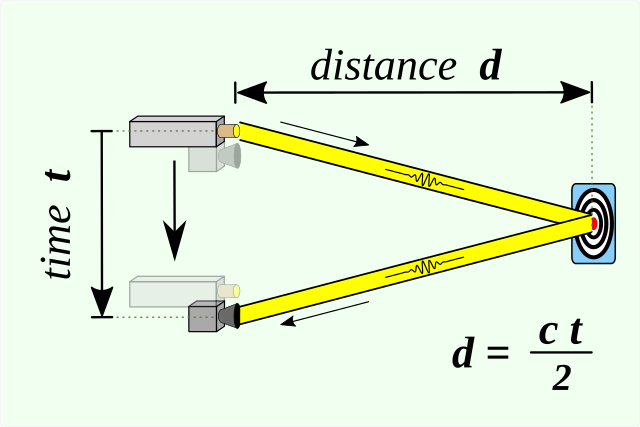
\includegraphics[width={0.5\textwidth}]{../assets/img/time_of_flight}
    \caption{Time of Flight~\autocite{wikipedia-contributors-2023D}}
\end{figure}
Dieses Konzept wird Time of Flight~\autocite{wikipedia-contributors-2023D}, kurz \textbf{ToF}, genannt und ist in Abbildung~\ref{fig:ToF} dargestellt.

Dem aufmerksamen Leser sollte aufgefallen sein, dass 4 weniger als 6 ist.
Deshalb können aus den 4 Zahlen auch nur 3DOF, also die Position, auf 0.3 bis zu 5 Meter genau, errechnet werden.

\subsubsection{Indoor Positioning System}\label{subsubsec:indoor-positioning-system}
Aufgrund dieser Ungenauigkeit kann GPS auch nicht für die ersten 3DOF genutzt werden.
Auch mit 30~cm ungenauigkeit könnten wir in keine virtuelle Realität eintauchen.

Deshalb müssen genauere Systeme her, sogenannte Indoor Positioning Systems~\autocite{wikipedia-contributors-2023E}.
Diese sind Systeme, die die Positionierung innerhalb eines Raums oder Arbeitsplatzes ermöglichen.
Ob 6DOF oder lediglich 3DOF erreicht werden ist dabei vom jeweiligen System abhängig.

\paragraph{Base Stations}\label{par:base-stations} werden hierfür klassischerweise verwendet.
Diese sind externe Geräte, welche, ähnlich wie die Satellite beim GPS, die Position des Empfängers ermitteln.

Es gibt einige enterprise Systeme, welche zum Beispiel in Lagerhäusern verwendet werden~\autocite{wikipedia-contributors-2023E}.
Für diese Ausarbeitung werden wir uns allerdings als Beispiel die SteamVR Base Station 2.0~\autocite{valve-corporation-no-date} anschauen.

Diese nutzen allerdings keine Time of Flight.
Anstatt die Position aus der Distanz zu errechnen wird hier die Position durch das Abtasten mittels eines Lasers ermittelt.
Damit werden mehrere markante Punkte an dem VR-Headset pro Basisstation abgetastet.
Es ergeben sich daraus also 6DOF\@.

\paragraph{Spatial cognition}~\autocite{wikipedia-contributors-2023F} ist die Warnehrung der Umgebung vom Menschen und anderen Lebewesen.
Unter anderem umfasst dieses Thema die Objektpermanenz.

Als ein bionischer Ansatz wird dieses Konzept heute auf AR-Headsets angewendet.
Daraus ergeben sich 6DOF, ohne an einen zuvor eingerichteten Raum gebunden zu sein.

\subsection{Spatial Cognition beim Menschen}\label{subsec:spatial-cognition-beim-menschen}
    \subsubsection{Proprioception}\label{subsubsec:proprioception}
    \subsubsection{Cognitive map}\label{subsubsec:cognitive-map}
    \subsubsection{Reference frames}\label{subsubsec:reference-frames}


\subsection{Spatial Cognition für AR-Headsets}\label{subsec:spatial-cognition-fuer-ar-headsets}
    \subsubsection{World Coordinate System}\label{subsubsec:world-coordinate-system}
    \subsubsection{Spatial anchors}\label{subsubsec:spatial-anchors}
    \subsubsection{Stationary frame of reference}\label{subsubsec:stationary-frame-of-reference}
        \paragraph{Knowledge engineering}~\autocite{wikipedia-contributors-2023C}